
\section{Stratégie de cette thèse (et du groupe CHIANTI)}%
\label{sec:stratégie__du_groupe_chianti}

\subsection{Place de ma thèse dans les problématiques de CHIANTI}%
\label{sub:place_de_ma_thèse_dans_les_problématiques_de_chianti}

Le groupe de recherche de chimie atmosphérique, neige, transfert et impacts (CHIANTI) au
sein duquel j'ai effectué ma thèse à l'IGE s'emploie ``à identifier les sources, les puits et
mécanismes de transformations des espèces chimiques générées par les activités humaines
(en particulier) afin de déterminer leur impact sur le climat, la composition et la
qualité de l’air, et les écosystèmes
enneigés''\footnote{\url{http://www.ige-grenoble.fr/-Chimie-atmospherique-CHIANTI-}}.
Le cadre de ma thèse concerne donc une sous partie de ces recherches, portant sur l'étude
de la qualité de l'air.

Une partie des travaux concerne un aspect fondamental de compréhension des processus
conduisant à la présence d'aérosols dans l'atmosphère, étudié par le biais de prélèvements sur le
terrain et d'analyses sur filtre effectuées par le plateau analytique Air-O-Sol à travers notamment
l'analyse de la fraction organique des PM (voir
section~\ref{sec:methodologie_de_prélèvement_et_d_analyse}).
Les mesures enregistrées dans la ``filtrothèque'' portent actuellement sur \num{18000}
filtres répartis sur plus de 80 sites différents et ont été possibles grâce à de très nombreux partenariats.

Ces partenariats avec les AASQUA ou d'autres instituts (LCSQA, INERIS, ADEME, ANSES...),
constituent également un volet important des recherches portant sur la réglementation et sur
la connaissance des processus et la quantification des sources d'émissions conduisant aux
concentrations de PM en air ambiant.
Différents programmes de recherche ont ainsi été élaborés en vue d'une amélioration de la
qualité de l'air (grâce au programme PRIMEQUAL par exemple) en appui à des plans de protections de
l'atmosphère (PPA). À titre d'exemple, l'importance
de la combustion de biomasse domestique en vallée alpine a pu être démontrée, conduisant
entre autres à la mise en place de la prime Air-bois, incitatif au remplacement des vieux
poêles à bois. Les conséquences de cette action ont été suivies et
analysées au sein du laboratoire depuis plusieurs années maintenant, avec le programme DECOMBIO~\autocite{chevrierDECOMBIOContribution2016,chevrierChauffage2016,allardQualite2018}.
Une liste des programmes ayant directement conduit aux données présentées dans cette thèse
est proposée en annexe~\ref{annexe:programmes_ayant_financés_la_thèses}.

Finalement, nous essayons aussi de nous rapprocher de l'impact sanitaire des PM à
travers le développement de méthodes d'analyse du potentiel oxydant (PO ou \textit{oxidative potential OP}) (voir
section~\ref{sub:potentiels_oxydants}). En plus du développement méthodologique de leurs
mesures, ces efforts du groupe ont porté sur l'analyse des PO sur plus de 45 sites de prélèvement différents, pour un
total de plus de 6500 échantillons pour lesquels le PO a été mesuré.
L'avantage majeur de la mesure du PO sur filtre consiste en la concomitance des mesures de
PO et de chimie, permettant des recherches couplées sur la chimie de l'aérosol et de son
potentiel oxydant, afin à terme de mieux comprendre la variabilité des différentes
mesures de quantification du PO et leurs liens avec d'autres variables métrologiques (par
exemple les connexions avec les déterminants géochimiques). Parallèlement, la pertinence de la
mesure du PO comme métrique sanitaire et sa comparaison avec la variable
réglementaire en vigueur (la concentration des PM) n'est pas encore totalement établie.
Les travaux du groupe sont donc également focalisés sur ce point, notamment par des travaux
pluridisciplinaires associant géochimistes et épidémiologistes.

\subsection{Méthodologie générale}%
\label{sub:méthodologie_general}

Ma thèse s'inscrit en plein cœur de ces thématiques du groupe de recherche et est transverse aux
différentes thématiques abordées, à savoir la détermination des sources d'émission d'intérêt
sanitaire.

Pour ce faire, la méthodologie générale suivante est donc adoptée et résumée sur le schéma
synthétique~\ref{fig:chapter01/workflow} :

\begin{enumerate}
    \item Grâce aux mesures de chimie et au modèle PMF, il s'agit de retrouver au mieux les
        sources d'émissions de PM;
    \item On entreprend ensuite de coupler les données issues de la PMF et les mesures de PO pour construire un
        modèle d'inversion permettant l'estimation de la contribution des différentes
        sources aux mesures des potentiels oxydants ;
    \item Ces résultats permettent ensuite de tenter d'estimer la variabilité géographique du potentiel oxydant des sources de PM.
\end{enumerate}

Chacun de ces items sera abordé dans des chapitres dédiés.

\begin{figure}[ht]
    \centering
    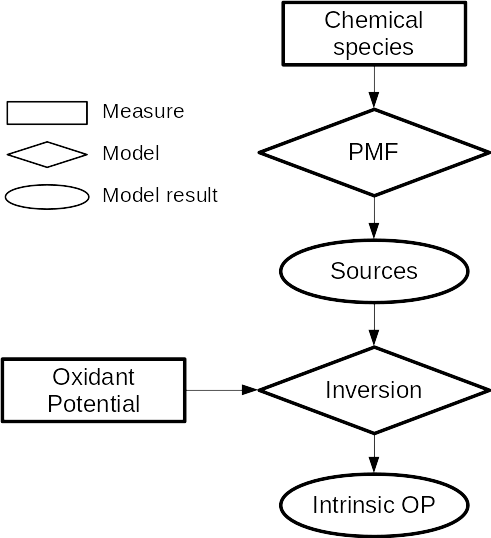
\includegraphics[width=0.5\linewidth]{chapter01/workflow.png}
    \caption{Méthodologie générale suivie au cours de cette thèse.}%
    \label{fig:chapter01/workflow}
\end{figure}


\subsubsection{Choix du modèle d'attribution de source}%
\label{ssub:choix_du_modèle_d_attribution_de_source}

Le choix du modèle source-récepteur PMF est motivé par son aptitude à reproduire les
concentrations locales sans préjuger a priori des spécificités du site de prélèvement. La
capacité du ME-2 à introduire des contraintes géochimiques est également un atout
important justifiant l'usage du modèle PMF.
Enfin, les précédents travaux au sein de l'équipe CHIANTI, en particulier ceux d'Antoine Waked, Benjamin Golly,
Florie Chevrier et Dalia Salameh sur le modèle PMF représentent également une expertise
appréciable justifiant le choix de cette méthode.

\subsubsection{Échantillons et analyses}%
\label{ssub:échantillons_et_analyses}

Les prélèvements, les mesures de concentrations des différentes espèces chimiques et les
mesures du PO s'appuieront sur les travaux préalables et en cours de l'équipe CHIANTI et
particulièrement ceux effectués sur le plateau analytique Air-O-Sol.
La base de données accumulées depuis plusieurs années est en construction permanente et mon travail sur son organisation est brièvement décrit ci dessous.

\subsubsection{PO et chimie ou PO et sources ?}%
\label{ssub:chimie_ou_sources_}

Le choix a été fait de ne pas utiliser directement les espèces chimiques comme prédicteur
des PO. En effet, sur la myriade d'espèces chimiques présentes sur les aérosols, seule une
partie infime est effectivement mesurée. Il n'est donc pas possible d'avoir une vue
exhaustive de la chimie des PM et l'attribution d'un PO intrinsèque par espèce chimique
présenterait nécessairement des biais du fait de corrélations entre une espèce mesurée mais
non redox-active (par ex. le lévoglucosan) et des espèces co-émises mais non mesurées (par ex. les
quinones). Quand bien même toutes les espèces seraient mesurées, on se retrouverait alors
avec un système d'équations avec beaucoup trop d'inconnues par rapport au nombre
d'observations (i.e jours de prélèvement), rendant caduque sa résolution.
A contrario, les facteurs PMF agrègent toute cette chimie en quelques variables, tout en
n'ayant besoin que de quelques espèces traceuses des émissions ou processus. Par exemple,
la combustion de biomasse est déterminée à partir de la présence de lévoglucosan. On pourra
donc attribuer un PO à la source \textit{combustion de biomasse}, avec concentration en PM
connue et un profil chimique déterminé (et partiellement inconnue), tout en ne sachant
pas exactement quelles espèces chimiques de cette source sont responsables de son PO.



\section{Methodologie de prélèvement et d'analyse}%
\label{sec:methodologie_de_prélèvement_et_d_analyse}

\subsection{Un filtre pour les gouverner tous}%
\label{sub:un_filtre_pour_les_gouverner_tous}

Les données utilisées pour cette thèse proviennent d'analyses faites en laboratoire à
partir de prélèvement de terrain (mesure \textit{off-line}) via des préleveurs
automatiques haut-volume, selon les recommandations de
l'EN~16450:2017~\autocite{cenAmbient2017a}, chaque prélèvement correspondant à une
journée d'échantillonnage. 

L'entiéreté des analyses des différents composés chimiques et de PO se fera sur ce même
filtre, dont différents morceaux seront prélevés, comme le montre la
figure~\ref{fig:chapter02/filter_speciation_en}.

\begin{figure}[ht]
    \centering
    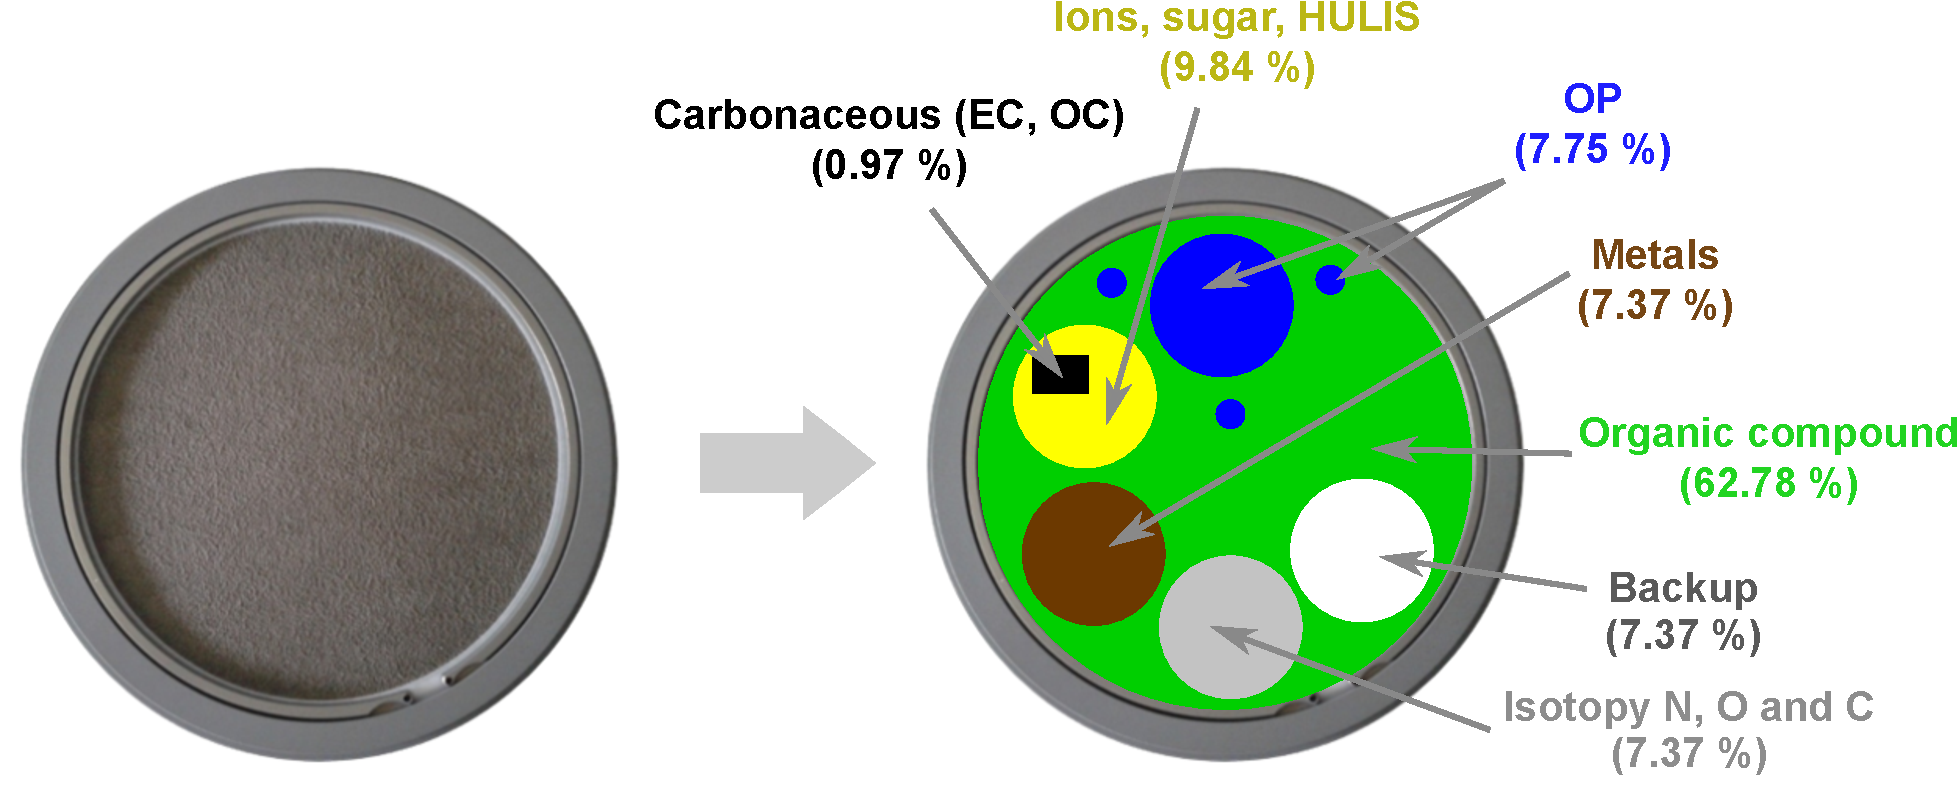
\includegraphics[width=1.0\linewidth]{chapter02/filter_speciation_en.pdf}
    \caption{Séparation typique des différentes surfaces de filtre pour préparation et
    analyses conduites à l'IGE ou dans les laboratoires collaborateurs.}%
    \label{fig:chapter02/filter_speciation_en}
\end{figure}

\subsection{Mesure des composés chimiques}%
\label{sub:analyses_des_composés}

\subsubsection{Préparation des filtres}%
\label{sub:préparation_des_filtres}

Les prélèvements sont réalisés sur des filtres en fibre de quartz pré-chauffés à
\SI{500}{\degreeCelsius} pendant 8 heures pour se prémunir de la présence en espèces
ioniques et organiques. Ces filtres sont chargés dans les porte-filtres des préleveurs
haut-débit (\SI{30}{\cubic\m\per\hour}) DA80 Digitel.

La fraction prélevée correspond très généralement aux \PMdix{} mais certains programmes
ont aussi considéré les \PMdc.
Les analyses réalisées sur ces filtres sont présentées brièvement ci dessous.

\subsubsection{Matière carbonée (EC et OC) : méthode thermo-optique}%
\label{ssub:matière_carbonnée_ec_et_oc_}

L’analyse de la matière carbonée (carbone organique (OC) et carbone élémentaire (EC)) est
réalisée directement sur un poinçon issu du filtre, à l’aide d’un analyseur
thermo-optique~\autocite[Sunset Lab. Analyser]{birchElemental1996}, par le protocole
EUSAAR-2~\autocite{cavalliStandardised2010,cenAmbient2017a}

Le principe de mesure est basé sur la détection par détecteur FID du \ce{CH4} issu de la
combustion puis réduction de la fraction carbonée présente dans l’échantillon. Une
fraction d'échantillon (1 ou \SI{1.5}{\centi\m\squared}) est placée dans un four en quartz
et soumise à différents plateaux de températures et sous des atmosphères plus ou moins
oxydantes. Une calibration journalière est effectuée. L’IGE participe annuellement à des
exercices d’intercomparaison dans le cadre du programme européen ACTRIS.

\subsubsection{Espèces ioniques : chromatographie ionique}%
\label{ssub:espèces_ioniques_par_chromatographie}

L'analyse de la fraction ionique des aérosols et des acides organiques légers est réalisée
sur la phase aqueuse (après extraction du filtre) par chromatographie
ionique~\autocite{jaffrezoSeasonal2005,cenAmbient2017b} (modèle Dionex ICS 3000) avec une
colonne
CS16 pour l’analyse des cations et colonne AS11 HC pour l’analyse des anions. L’analyse
des anions permet la quantification des ions chlorure \ce{Cl-}, nitrate \ce{NO3-} et
sulfate \ce{SO4^2-}. L’analyse des cations permet la quantification du sodium \ce{Na+}, de
l'ammonium \ce{NH4+}, du potassium \ce{K+}, du magnésium \ce{Mg^2+} et du calcium
\ce{Ca^2+}. 
Les concentrations en oxalate et en acide méthane sulfonique (MSA) sont aussi accessibles.
La calibration est réalisée tous les jours à partir de solutions standards certifiées.

\subsubsection{Sucres et autres polyols : HPLC-PAD}%
\label{ssub:sucres_et_autres_polyols_hplc-pad}

L’analyse de la fraction soluble des sucres et des polyols est réalisée sur la phase
aqueuse, par une méthode HPLC avec détection par PAD (Pulsed Amperometric Detection)
(modèle Thermo 5000+) avec des colonnes Metrosep (Carb 1 – Guard+A Supp 15 – 150+Carb
1 – 150)~\autocite{piotQuantification2012,wakedSource2014}.
Cette analyse permet la quantification des saccharides anhydrides (lévoglucosan,
mannosan, galactosan) et des polyols (xylitol, arabitol, sorbitol, mannitol) et sucres
(glucose). La calibration est réalisée tous les jours à partir de solutions standards.
L’IGE a participé dernièrement à une intercomparaison européenne des mesures de
lévoglucosan.

\subsubsection{Cellulose : digestion enzymatique et HPLC-PAD}%
\label{ssub:cellulose_}

La cellulose est mesurée par un protocol améliorant celui de \cite{kunitEnzymatic1996}.
La cellulose est extraite en solution aqueuse, puis l'extraction est faite dans
différentes solutions ensymatique afin de digèrer la cellulose en glucose. Le glucose est
ensuite mesuré par HPLC-PAD.

Brievement, un poiçon de \SI{21}{\mm} de diamètre est extrait du filtre dans un bain à
ultra-son pendant \SI{40}{\minute} dans une solution aqueuse de \SI{3}{\ml} tamponé à pH
4.8 par un buffer au thymol. Deux solutions enzymatiques (cellulase (Sigma Aldrich, C2730)
avec \SI{20}{\ul} de solution aqueuse à \SI{70}{unit.\g^{-1}} et glucosidase (Sigma
Aldrich, 49291), avec \SI{60}{\micro\L} de solution aqueuse à \SI{5}{unit.\g^{-1}}) sont
ajoutées. La solution est incubée à \SI{50}{\degreeCelsius} pendant \SI{24}{h} pour
hydrolyse. L'hydrolyse est arrếtée par chauffage au four à \SI{100}{\degreeCelsius}
pendant \SI{45}{min}. La solution est ensuite centrifugée (\SI{7000}{rpm}) pendant
\SI{15}{min} et extraite par seringue pour analyse en HPLC-PAD.

L' HPLC-PAD (Dionex DX500) est équipée d'une colonne Methrom (\SI{250}{mm} de long,
\SI{4}{mm} de diamètre) par un run isocratique de \SI{40}{min} avec les éluants 
A (\SI{50}{\percent}, \SI{18}{nM} \ce{NaOH}), B (\SI{25}{\percent}, \SI{100}{nM} \ce{NaOH} + \SI{150}{nM}
\ce{NaAc}) et C (\SI{25}{\percent}, \SI{220}{nM} \ce{NaOH}). La température de la colonne
est maintenue à \SI{30}{\degreeCelsius}. Le débit d'éluant est fixe à
\SI{1}{\ml\per\minute} et le volume d'injection de \SI{250}{\ul}.
À chaque lot d'analyse est également inclus une solution standard de glucose et de
cellulose (perles de \SI{20}{\um}, Sigma Aldrich, S3504) analysées selon le même
procédé que les échantillons afin de déterminer l'efficacité spécitique de la conversion
enzymatique cellulose-glucose. Le calcul de la concentration finale de cellulose libre
prend en compte ce ratio de conversion, variant entre les lots entre
\SIrange{65}{80}{\percent}.
À cette concentration est soustraite la concentration initiale en glucose, mesurée
parallèlement par HPLC-PAD (décrite section~\ref{ssub:sucres_et_autres_polyols_hplc-pad}).
Enfin, la mesure des blancs de terrains et de laboratoire sont également pris en compte
dans cette mesure.

\subsubsection{Acides organiques légers : HPLC-MS}%
\label{ssub:acides_organiques_légers_hplc_ms}

L’analyse de la fraction soluble d’une vingtaine d’acides organiques légers (C2 – C7) est
réalisée sur la phase aqueuse, par une méthode HPLC avec détection par Spectrométrie de
Masse (Dionex DX500 + MS LCQ Fleet Thermo) avec séparation sur une colonne Waters
Carotenoid. Cette analyse permet la quantification d’une assez large série d'acides
organiques (depuis l’oxalate jusqu’à l’acide benzoïque). Ces acides sont issus de
processus d’oxydation de matière organique d’origine biogénique ou anthropique. La
calibration est réalisée tous les jours à partir de solutions standards.

% Analyses des HULIS par TOC
% L’analyses de la fraction soluble dans l’eau des HULIS (Humic-Like Substances ;
% composés macromoléculaires polyfonctionnels polyacides) est réalisée par une séparation
% avec filtration sur résine DEAE, permettant de ne retenir que les HULIS de
% caractéristiques précises, tout en éliminant les autres espèces solubles de la matière
% carbonée. Ces HULIS sont ensuite élués de cette résine, l’échantillon récupéré étant
% ensuite analysé pour son contenu en carbone total avec un analyseur Shimadzu TOC 5000.
% Les protocoles détaillés ont été mis au point dans le cadre de la thèse de C Baduel (cf
% Hal CNRS).

% Préparation et analyses de traceurs organiques par GC-MS :
% Ces analyses sont réalisées au LCME (Chambéry). Pour réaliser la spéciation
% moléculaire, une fraction de filtre est extraite par extraction solide/liquide
% filtre/solvants organiques (acétone/dichlorométhane 1:1) à 100°C et 100 bar à l’aide
% d’un Accelerated Solvent Extractor (ASE 200 – Dionex). L’extrait est ensuite concentré
% grâce à un évaporateur (TurboVap II – Zimark) puis filtré à 0,1 µm (Anotop 10 –
% Whatman), Cet extrait est ensuite divisé en fractions pour l’analyse de 15 HAP, de
% composés polaires (entre autres de nombreux dérivés de la combustion de la biomasse,
% etc), et de composés apolaires (alcanes C11 à C40 et 10 hopanes), soit environ une
% grosse centaine d’espèces organiques.

% L’analyse des deux dernières séries de composés est réalisée par GC-MS (chromatographie
% gazeuse couplée à un spectromètre de masse ; GC Clarus 500 associée à un MS 560 –
% Perkin Elmer). Pour les composés polaires, avant l’analyse par GC-MS, l’extrait est
% dérivé par ajout du NO-Bis(trimethylsilyl)trifluoroacetamide (BSTFA) + 1% de
% trimethylchlorosilane (TMCS) en proportion 1:1 v/v et sous agitateur chauffant à 50°C
% pendant deux heures. La quantification est réalisée sur des fragments caractéristiques, la
% calibration étant réalisée à partir de solutions standards et de la méthode à l’étalon
% interne deutéré (n-dodecane d26 pour les composés apolaires et levoglucosan d7 pour les
% composés polaires). La bibliothèque de spectre utilisée est la NIST 2001.

% Analyses des HAP :
% L’analyse des HAP est réalisée par HPLC-fluorescence (chromatographie liquide couplée à
% un détecteur par fluorescence ; HPLC de type Series 200 couplée à un détecteur de type
% Series 200a – Perkin Elmer). La colonne de séparation est une colonne de type phase
% inverse C18 (NUCLEOSIL 100-5 C18 PAH, 25cm × 4,6 cm) éluée avec une phase mobile formée
% d’un mélange méthanol/eau en mode gradient. Cette méthode permet l’analyse des 13 HAP
% classés prioritaires par l’US-EPA (Phénanthrène, Anthracène, Fluoranthène, Pyrène,
% Benzo[a]anthracène, Chrysène, Benzo[e]pyrène, Benzo[b]fluoranthène,
% Benzo[k]fluoranthène, Benzo[a]pyrène, Benzo[ghi]pérylène, Dibenzo[a,h]anthracène,
% Indéno[1,2,3-cd]pyrène) ainsi que du rétène et du coronène. Le LCME a participé aux
% dernères intercomparaisons mises en place par le LCSQA.

\subsubsection{Métaux et traces : IPC-MS ou AES}%
\label{ssub:métaux_et_traces}

Les analyses sont réalisées dans un laboratoire qui
participe aux exercices d’intercomparaison organisés par les Mines de Douai. Ces analyses
sont réalisées par ICP-MS après digestion acide (ou ICP-AES selon les sites
d'études)~\autocite{allemanPM102010,mbengueSizedistributed2014,cenAmbient2005}.
Les métaux et éléments traces analysés sont compris dans la liste suivante : Al, Ag, As,
Ba, Be, Br, Bi, Ca, Cd, Ce, Co, Cr, Cs, Cu, Fe, K, La, Li, Mg, Mn, Mo, Na, Ni, Pb, Pd, Pt,
Rb, Sb, Sc, Se, Sn, Sr, Ti, V, Zn et Zr.

\subsection{Mesure des potentiels oxydants}%
\label{sub:potentiels_oxydants}

Le PO acellulaire des aérosols est déterminé par la capacité intrinsèque des particules
atmosphériques à oxyder le milieu pulmonaire en générant/induisant la formation de ROS.
Les différents filtres seront soumis à deux tests de PO complémentaires, choisis pour
leur représentativité (dénommés PO DTT, et PO AA en fonction du substitut de
l’antioxydant pulmonaire impliqué dans le test, le Dithiotréitol (DTT) et l’acide
ascorbique (AA)). 

Pour chacun des deux tests présentés ci-après, des triplicats de mesures sont effectués, un
témoin positif à la 1,4-naphtoquinone est utilisé et les blancs de laboratoire sont
soustraits aux échantillons.

\subsubsection{Prendre en compte la bioaccessibilité: SLF}%
\label{sub:prendre_en_compte_la_bioaccessibilite_slf}

Étant donné que l'on cherche à reproduire le comportement des PM en milieu biologique
(les poumons), il est important de procéder à l'extraction et l'analyse du PO dans un
fluide reproduissant au plus fidèlement possible ce milieu, et non directement dans de
l'eau milli-Q.

Il existe différents types de fluides mimiant les surfactants pulmonaires
(\textit{simulated lung fluid} (SLF)). Les analyses de cette thèse ont toutes été
réalisées selon le du protocole de \textcite{calasPollution2017} et pour lequel il est fait
usage d'un mélange de solution de Gamble+DPPC.  \textcite{calasImportance2017} ont pu
montrer que différents SLF produisent des mesures de PO sensiblement différentes.
Notamment, l'ALF tend à produire des mesures de PO systèmatiquement inférieures à la
mesure faite dans du Gamble+DPPC (2 à 3 fois plus faible), qui elle-même est légèrement
inférieure à la mesure faite dans de l'eau milli-Q.

\subsubsection{Mesure au dithiothréitol (DTT)}%
\label{ssub:mesure_au_dtt}

L’objectif du test DTT est de suivre la cinétique de consommation du dithiothréitol (DTT)
par des espèces redox-actives portées ou générées en présence de PM. Le dithiothréitol,
réactif principal du test, qui a donné son nom à l’expérience par extension, est un thiol
qui présente un fort pouvoir réducteur (E°=\SI{0.33}{\V}) équivalent à celui d’agents réducteurs
biologiques. Il est considéré comme un substitut aux antioxydants pulmonaires.

Le suivi cinétique se fait par titration à intervalles réguliers (0, 15 et 30 minutes) du DTT
restant (i.e. non oxydé), par réaction avec le DTNB (acide
5-5'-dithiobis-2-nitrobenzoïque). Le produit de réaction, le thionitrobenzoate (TNB) de
couleur jaune, permet la quantification par suivi d'absorbance à \SI{465}{nm}.

Initialement utilisé par~\textcite{choRedox2005} pour mesurer une concentration simulée de
\ce{O2^{.-}} engendrée par la présence de composés organiques, il a été ensuite montré par
\textcite{beiReaction2014} que le DTT est potentiellement sensible à une plus grande
variété de ROS qu'imaginé dans le schéma réactionnel originel. C'est maintenant le test le
plus largement utilisé pour mesurer le PO des PM, notamment grâce à la simplification et
la semi-automatisation de ce test par \textcite{fangSemiautomated2015}.

Il a été montré également que ce réactif n'est pas sensible qu'aux composés organiques
mais également aux métaux~\autocite{charrierDithiothreitol2012,linGeneration2011}.

Ce test est cependant limité du fait que le DTT n'est pas capable de mesurer
\ce{HO^{.}}, qui est pourtant l'un des ROS prépondérants~\autocite{xiongRethinking2017}.

\subsubsection{Mesure à l'acide ascorbique (AA)}%
\label{ssub:mesure_à_l_aa}

Ce test, initié par \textcite{zielinskiModeling1999} pour mesurer la capacité oxydante de
particules fines issues de la combustion de diesel, puis adapté par
\textcite{mudwayVitro2004,ayresEvaluating2008}, utilise l'acide ascorbique (AA) comme
anti-oxydant.
L'acide ascorbique ou vitamine-C est un anti-oxydant naturellement présent au niveau du
surfactant pulmonaire. De la même manière que pour le test au DTT, l'AA est oxydé par
les ROS des PM.

Le suivi cinétique de la consommation de AA se fait pas absorbance à \SI{265}{\nano\m}
toutes les 4 minutes à partir de la deuxième minute, pendant 30 minutes au total.

Le test AA est reconnu pour sa forte réactivité vis-à-vis des métaux de transition. 


% \subsubsection{Mesure par DCFH}%
% \label{ssub:mesure_par_dcfh}
%
% Le test DCFH mesure de façon acellulaire le potentiel oxydant des particules en suivant
% par fluorescence l’oxydation d’un composé par les ROS produits ou véhiculés par les PM en
% présence.
%
% L’oxydation de la DCFH (dichlorofluorescéine) conduit à la DCF (2’,7’dichlorofluorescéine)
% qui est fluorescente. Le dosage de la dichlorofluorescéine est communément utilisé en
% biologie pour visualiser la génération de ROS (reactive oxygen species) mais aussi de RNS
% (reactive nitrogen species) à un niveau intracellulaire et acellulaire. C’est donc un test
% qui va réagir avec plus d’espèces et qui est moins spécifique que les tests DTT ou AA qui
% ne mesurent que les ROS. Il est néanmoins très complémentaire.
%

\subsubsection{Unités de mesure}%
\label{ssub:unitees_de_mesures}

La mesure du PO par DTT ou AA fournit une consommation de réactant en \si{\nmol\per\minute}.
Cependant, cette mesure est nécessairement dépendante de la quantité de PM introduite dans
la réaction.
Il convient donc de normaliser cette consommation d'antioxydant par la masse des réactifs.
Seulement, cette mesure n'est pas fidèle à l'exposition des personnes car ne prend pas en
compte la variabilité des concentrations en particules dans l'air. De ce fait, deux normalisations de la réactivité des
particules par la mesure du PO coexistent.

\paragraph{Normalisation par la masse}%
\label{par:normalisation_par_la_masse}
Pour exprimer la réactivité ``intrinsèque'' d'un ensemble de particules, la cinétique de déplétion
d'antioxydant ($cAO$, en \si{\nmol\per\minute}) est normalisée par la masse de réactif
introduit (en \si{\ug}). On obtient ainsi le PO par \si{\ug}, noté \OPm{} en
\si{\opm}:
\begin{align}
    \label{eq:opm}
    OP_m &= \frac{cAO - cAO_{blank}}{M}
\end{align}
où $cAO$ est la consommation d'antioxydant dans l'échantillon et $cAO_{blank}$
est la consommation d'antioxydant dans les blancs, tous deux en \si{\nmol\per\minute}, et $M$
la masse de réactif introduit (PM ou élément chimique), en \si{\ug}.

\paragraph{Normalisation par le volume}%
\label{par:normalisation_par_le_volume}

Seule, la réactivité intrinsèque n'est pas un indicateur propice à évaluer
l'exposition des personnes. En
effet, il faut également tenir compte de la concentration ambiante des particules. Le PO
est donc aussi exprimé par unité de volume, notée \OPv{} en \si{\opv} et parfois appelé PO
``extrinsèque'', calculé par:
\begin{align}
    \label{eq:opv}
    OP_v &= OP_m \times [\text{PM}]
\end{align}
où [PM] correspond à la concentration en particule en \si{\ugm}. Cette expression se
retrouve également écrite~\autocite{fangSemiautomated2015} sous la forme
\begin{align}
    \label{eq:opvalt}
    OP_v &= \frac{cAO - cAO_{blank}}{V}
\end{align}
où $V$ est le volume d'air analysé. Ces deux formes sont cependant équivalentes, car en
replacant $V = \frac{M}{[PM]}$ dans l'Eq.~\ref{eq:opvalt}, on retrouve bien
l'Eq.~\ref{eq:opv}:
\begin{align}
    \label{eq:opvopvalt}
    OP_v &= \frac{cAO -cAO_{blank}}{V} = \frac{cAO -cAO_{blank}}{M}\times [\text{PM}] = OP_m \times [\text{PM}].
\end{align}

\paragraph{Comparabilité des échantillons}%
\label{par:comparabilité_des_échantillons}

Le fait de se ramener à un microgramme de PM en divisant par la masse introduite fait
l'hypothèse d'une linéarité du PO en fonction de la masse sur une large gamme de mesure. Or, il a été montré par
\textcite{charrierDithiothreitol2012,charrierBias2016,calasComparison2018} que cette
hypothèse est fausse dans le test au DTT, test qui présente en réalité une réponse
pseudo-logarithmique en fonction de la masse du réactif.

Ainsi, deux analyses du même filtre ne présenteront pas la même valeur de \PODTTm{} si la
concentration en PM utilisée pour le test n'est pas identique : les analyses faites à ``fortes masses''
présenteront toujours un \PODTTm{} plus faible que celles à ``faibles masses''.
La comparabilité des échantillons n'est donc possible que si les analyses sont faites à
masses constantes, ou artificiellement corrigées, soit par interpolation, soit par
estimation grâce à la concentration de Cu et Mg, comme le proposent
\textcite{charrierBias2016}.

Il faut également noter que ce biais se propage au \PODTTv{} du fait de sa linéarité avec le
\PODTTm. Aussi, un deuxième biais apparaît ici. En effet, la non-linéarité de la réponse
du test DTT fait
que la prolongation linéaire entre 1 microgramme et X microgrammes par mètre cube est
fausse.
% Le \PODTTv{} se comportant alors ``comme si'' les X microgrammes de PM de ce mètre
% cube d'air se comportaient comme X fois 1/X 1 microgramme de PM, ce qui est faux de part
% la non-linéarité du test DTT.

Les analyses de \PODTT{} de cette thèse suivent donc le protocole défini dans le groupe lors de la thèse
de \textcite{calasPollution2017} : analyse à masse constante et faible de PM. Les
échantillons seront donc comparables entre eux. Le parti pris de garder le biais
d'extrapolation de la ``faible masse'' à un volume d'air potentiellement chargé en PM
pour le \PODTTv{} se justifie biologiquement par les faibles volumes d'air présents dans les
poumons et donc la faible masse de PM en contact avec les surfactants pulmonaires à
chaque inspiration\footnote{Du moins pour les gammes de concentrations observées
communément en Europe.}.

Une telle non-linéarité n'est pas observée pour les tests à l'acide ascorbique.

Les résultats de cette thèse issus de ces tests sont donc à priori comparables entre tous les
échantillons mesurés dans les différentes études.


\section{Signature chimique des facteurs PMF}%
\label{sec:signature_chimique_des_facteurs_PMF}

Chaque source d'émission n'émettant pas les mêmes composés, une analyse chimique
des PM permet l'estimation des contributions des différentes sources aux PM observés.
Seulement, il n'est pas possible de mesurer l'entièreté des plusieurs milliers d'espèces chimiques
présentes dans les aérosols.
Il convient donc de connaître au mieux la signature chimique des différentes sources
d'émissions, notamment via des prélèvements à l'émission en condition
réelle ou en chambre d'étude. La connaissance des espèces spécifiquement émises ou des
ratios d'émissions entre différentes espèces des différentes sources permettra par la
suite l'attribution de la contribution de ces sources aux PM observées.

\subsection{Profil chimique des sources d'émissions courantes}%
\label{sub:profil_chimique_des_sources_d_émissions_courantes}

\begin{description}
    \item[Combustion de biomasse] provenant en Europe majoritairement du chauffage
        domestique. Le type de combustible et les conditions de combustion influencent
        grandement les espèces chimiques émises. On retrouve cependant toujours de
        l'OC en grande quantité, ainsi que de l'EC. Aussi, si le BC est mesuré, il est
        possible d'estimer la part du BC provenant de cette source de combustion \BCwb{}
        (\textit{BC wood burning}), en particulier avec des mesures réalisées par
        aethalomètre AE33.
        Provenant de la pyrolyse de la cellulose, le lévoglucosan, le mannosan et
        le galactosan forment trois traceurs spécifiques de cette source, car il n'existe
        pas d'autre procédé connu conduisant à leur présence dans l'atmosphère que la
        combustion de
        bois~\autocite{jordanLevoglucosan2006,puxbaumLevoglucosan2007}.
        Enfin, du potassium \ce{K+} et du rubidium Rb sont également associés à cette
        source~\autocite{navaBiomass2015,gollyEtude2014,chevrierChauffage2016}.

    \item[Trafic routier] émettant différents métaux (Ca, Cu, Mo, Pb, Sb, Sn, Fe, Zr,
        Ti) et de la matière carbonée --notamment de l'EC-- et des composés organiques
        (hopanes, alcanes)~\autocite{schauerCharacterization2006,charronIdentification2019}. Les émissions
        véhiculaires peuvent être séparées en deux sous-types : émissions à l'échappement
        provenant de la combustion~\autocite{allenSize2001,huMetals2009,vianaSource2008},
        et émissions hors-échappement (abrasion de la route, usure des freins et pneus,
        etc.)~\autocite{grigoratosBrake2015,sandersAirborne2003,sternbeckMetal2002}.
        Une partie des composés gaseux (COV et \ce{NO_x}) émis par cette source peuvent
        également conduire à la formation de particules secondaires.

    \item[Émissions primaires biogéniques] directement émises par les micro-organismes du sol
        et des plantes, qui, de par leur activité biologique, émettent notamment
        différents polyols : arabitol, mannitol,
        sorbitol~\autocite{bauerSignificant2008,yttriAmbient2007,samakePolyols2019}. De
        très nombreuses autres sources primaires biogéniques sont possibles (émissions de
        pollen, de débris végétaux, etc.) \autocite{samakePolyols2019}.

    \item[Poussière crustale] remise en suspension par le vent ou les activités humaines
        (mine, carrière, etc.). Ce profil chimique reflète en grande partie celui de la croute continentale
        et présente donc du Mg, Ca, Ti, Mn et Fe, mais très peu de composés
        organiques~\autocite{almeidaSource2005,dallostoHourly2013,morenoVariations2011,putaudSizesegregated2004}.

    \item[Sel de mer] issue des embruns marins, présentant donc une grande proportion de
        \ce{Na+} et \ce{Cl-}, mais également de
        \ce{Mg^2+}~\autocite{belisCritical2013,odowdMarine1997,pioClimatology2007}. Il
        est à noter que le sel de déneigement, notamment en vallées alpines, présente la même
        composition chimique~\autocite{airrhone-alpesInfluence2012}.

    \item[Industrie] très variables car dépendent directement du type d'industrie.
        Cependant, il est courant d'y retrouver des métaux, du \SOq{} et certains composés
        organiques spécifiques (HAP et HAPS, hopanes...) selon les procédés
        industriels~\autocite{elhaddadPrimary2011,sylvestreComprehensive2017}.

    \item[Port et bateau] proche des côtes notamment. Marqué par la présence de V et Ni,
        provenant de la combustion de fuel lourd, mais également de composés organiques
        comme les hopanes.

    \item[Agriculture] émettant notamment du nitrate et de l'ammoniac à travers les
        fertilisants de synthèse ou de fumier. Cette source d'émission est notamment
        responsable des pics de pollution printaniers, lors des épandages agricoles à cette
        période.

    \item[Volcan] beaucoup plus ponctuel --surtout en Europe-- mais néanmoins possible
        (par exemple l'Eyjafjöll en 2010), les volcans émettent de grandes quantités de
        poussières minérales et d'éléments traces, mais également de soufre que l'on
        retrouvera sous forme de \SOq.

\end{description}

\subsection{``Sources'' ou processus secondaires}%
\label{sub:_sources_secondaires}

Aux sources primaires précédemment listées, il faut ajouter les processus secondaires liés
à la photochimie ou au vieillissement des aérosols, qui conduisent à la formation de
nouvelles espèces chimiques.

\paragraph{Aérosol organique secondaire}%
\label{par:aérosol_organique_secondaire}

Notamment, la biologie est connue pour émettre de très grandes quantités de Composés
Organiques Volatils (COV ou \textit{volatil organic carbon VOC}) qui vont conduire à la
formation d'une myriade d'aérosols organiques secondaires (AOS, ou \textit{secondary
organic aerosols SOA}). C'est le cas des émissions de terpènes, de l'isoprène,
mais aussi du dimethyl sulfate (DMS), s'oxydant en
MSA dans l'atmosphère. Sa présence dans les PM trace donc le vieillissement d'un aérosol
d'origine organique. De très nombreuses familles d'espèces résultent aussi des émissions
de COV anthropiques.  
L'oxalate est également un composé issu de réactions photochimiques,
mais la diversité des composés primaires et voies de réaction rendent extrêmement difficile
l'identification des sources originelles.
On nomme alors tous ces aérosols \textit{secondary organic aerosol} (SOA), dont le
dénominateur commun est de présenter une fraction importante de matière organique
oxygénée. Il est compliqué avec des analyses moléculaires d'en déterminer l'origine et
quelques travaux sont en cours dans le groupe en ce sens (parmi une multitude d'autres
dans la communauté de recherche sur les aérosols) et présentés dans le
chapitre~\ref{cha:approfondissement_des_connaissances_des_sources_des_pm}.

Il faut noter que d'autres techniques d'analyses, notamment via des mesures de
spectrométrie de masse en ligne dans l'atmosphère, permettent une
analyse plus avancée de cette fraction organique de l'aérosol, sans pour autant pouvoir
caractériser moléculairement les espèces retrouvées.

\paragraph{Aérosols inorganique secondaire}%
\label{par:aérosols_inorganique_secondaire}

Mais la partie organique n'est pas la seule à réagir dans l'atmosphère. Ainsi, les
\ce{NO_x}, gazeux, émis notamment par le transport routier, peuvent condenser en phase
particulaire lorsqu'ils s'associent à l'ammoniac, provenant du secteur agricole, pour
former du nitrate d'ammonium \ce{NO3NH4}. Il en est de même pour le \ce{SO2} émis par
différentes sources ou des fonctions sulfatées de la matière organique, et l'ammoniac,
condensant en sulfate d'ammonium \ce{SO4(NH4)2}. Cependant, une part de cet aérosol
inorganique tracé par le sulfate d'ammonium présente une part non-négligeable de OC mais
aussi du Sélenium \ce{Se}, en faisant un facteur mixte inorganique et organique. Des travaux
sur ce facteur sont présentés dans le
chapitre~\ref{cha:approfondissement_des_connaissances_des_sources_des_pm}.

\paragraph{Vieillissement et volatilité}%
\label{par:vieillissement_et_volatilité}

Aussi, la partie la plus volatile de la phase particulaire tend à s'évaporer et rejoindre
la phase gazeuse au cours du temps. C'est ainsi qu'après plusieurs jours de transport
dans l'atmosphère, le sel de mer peut avoir ``dégazé'' le chlore présent dans son réseau
cristallin, et présenter des substitutions avec du sulfate ou du
nitrate~\parencite{chiSea2015}. De même que le
sodium peut avoir été remplacé par d'autres cations comme le potassium ou le magnésium.
Souvent, ce procédé est associé à une augmentation de la matière organique liée à cet
aérosol.


\section{Harmonisation et gestion de base de données}%
\label{sec:harmonisation_et_gestion_de_base_de_donnée}

\subsection{Problématique : des quantités de plus en plus conséquentes}%
\label{sub:problématisation_des_quantités_de_plus_en_plus_conséquentes}

Pour approfondir la compréhension de la chimie des PM, la base de données accumulée à l'IGE
est extrêmement précieuse par son ampleur et sa diversité de lieux et chimie analysée.
Seulement, jusqu'à présent, la généralisation d'observation était rendue compliquée par une
difficulté technique : chaque série d'analyse était enregistré sur des supports différents,
sans standardisation et avec des méta-données partielles. Cela ne posait pas de problème
tant que la personne en charge de l'étude de ces séries de mesure avait une connaissance
implicite du jeu de données et tant que la quantité d'analyses était restreinte.

Cependant, l'accumulation de mesures provenant de différents programmes de recherche et la
diversité des personnes ayant à traiter ces résultats ainsi qu'une volonté de synthèse
a demandé un travail de fond sur la gestion de cette base de données afin de la rendre 
homogène (même unité, même nomenclature, même format de date…) et intercomparable
(métadonnées complètes : fraction des PM analysée, site de prélèvement, date et heure du
début et fin de prélèvement…).

Aussi, le volume de données généré, sans être à proprement parler du \textit{big data}
\footnote{Bien qu'il n'y ait pas de définition formelle de \textit{big data}…  Une
    définition que j'apprécie stipule que le \textit{big data} commence lorsque tout
    n'est plus visible sur un tableur. Dans ce cas, nous pouvons catégoriser cette base de
donnée de \textit{big data}.},
demande un traitement automatique de diverses vérifications (balance ionique, détection
d'erreur de mesure…) et pré-calcul de variables d'intérêts (bilan de masse des PM,
fraction crustale…).

La quantité de données génère aussi un besoin de visualisation rapide de ces mesures et
d'outils de statistique exploratoire uni- ou multi-variées rapides d'utilisation
(corrélation, dispersion saisonnière, comparaison entre sites…) tant pour la vérification
des mesures (analyse de points sortant de l'ordinaire…) que pour des recherches
préliminaires (cycle saison de telle espèce chimique sur sites côtiers ou alpins, évolution
inter-annuelle, ratio lévoglucosan/OC…).

Aussi, et c'est la raison originale pour laquelle je me suis attaché à cette
problématique, le croissement de l'ensemble des mesures n'était pas possible. La question
s'était posée initialement de connaitre les filtres présentant une concentration d'OC
élevée associés à une concentration de sélénium importante pour une possible collaboration
du groupe de recherche \parencite{toluDistribution2014,luxemStudying2017}.

Enfin, il n'existait pas de gestion de sauvegarde ou de suivi de l'édition
de chacun de ces fichiers, rendant ces mesures dépendantes d'un seul support.

\subsection{Mise en place et gestion d'une base de données pour la filtrothèque}%
\label{sub:mise_en_place_et_gestion_d_une_base_de_donnée_pour_la_filtrothèque}

\begin{tcolorbox}[colback=red!5!white,colframe=Melon,title=Note]
Ma thèse ayant re-mobilisée directement dans mes travaux ou dans des travaux associés de
très nombreuses mesures, une des premières étapes de mon travail a consisté en la mise en place d'une
base de données centralisée et homogène de la filtrothèque, pouvant ainsi être traitée de
manière automatisée.
\end{tcolorbox}

L'ensemble des actions nécessaires et des procédures mises en place pour la gestion des
données dans le groupe est présenté dans le schéma~\ref{fig:bdd}.

\paragraph{Différents usages et utilisateurs}%
\label{par:différents_usages_et_utilisateurs}

Les contraintes majeures suivantes devaient être respectées :
\begin{enumerate}
    \item facilité d'utilisation pour la diversité des techniciens et techniciennes du
        plateau analytique,
    \item suivi, sauvegardes et historisation des mises à jour,
    \item standardisation, structuration et interopérabilité vers différents logiciels ou
        langages de traitement (python, R, QGIS…).
\end{enumerate}
Le point numéro 1 demande donc une interface haut niveau (copier/coller, cliquer et
éditer, commentaire, mise en couleur…) typique d'un tableur, alors que le point 3 plaide
davantage pour des formats de bases de données plus élaborés (SQL, HDF…).
Aussi, différents fichiers doivent pouvoir être mis en relation (lien site et
échantillon, méta-données du
filtre et résultat d'analyse, résultat PMF et échantillon…), ce qui est très bien géré
par le langage SQL. Aussi, les \textit{dump} des bases de données SQL peuvent s'historiser
de façon incrémentale tout en permettant de retrouver très exactement la base de données à
n'importe quelle date. 
Pour l'instant, le choix du stockage s'est donc porté sur \textit{sqlite} pour sa
simplicité d'utilisation\footnote{Cependant, le problème majeur de sqlite réside en son
    absence de serveur accessible depuis l'extérieur. Une évolution possible serait un
serveur postgres ou mysql.}.

\paragraph{Historisation et stockage}%
\label{par:historisation_et_stockage}

L'historisation sera quant à elle gérée par un gestionnaire de version. Ici, \textit{git}
est choisi. La sauvegarde se fera en local sur les serveurs de l'IGE, mais également sur
un dépôt git de l'université\footnote{Dépôt git :
\url{https://gricad-gitlab.univ-grenoble-alpes.fr/pmall/bdd_aerosols}} (dépôt non
public car certaines données ne sont pas publiques).
Techniquement, l'historisation se fait par un versionnage d'un export de la base de
données en
SQL --afin de pouvoir reconstruire l'intégralité de la base de données-- ainsi qu'en
l'export en CSV de chacune des séries de mesures par site d'étude.

\paragraph{Harmonisation et pré-calcul}%
\label{par:harmonisation_et_pré_calcul}

Plusieurs variables d'intérêts sont souvent demandées, telles que la part crustale, la
somme des certains polyols, l'estimation de la masse des PM reconstruite par bilan de
masse… Aussi, ces variables sont donc automatiquement calculées en fonction des données
disponibles. À titre d'exemple, la masse estimée des PM par bilan de masse est nécessaire
pour la mesure du PO à masse de PM constante. Seulement, les estimations des différentes
parties (crustale, sel marin, etc) peuvent dépendre des espèces mesurées, rendant complexe
leur estimation.

\begin{landscape}
\begin{figure}[ht]
    \centering
    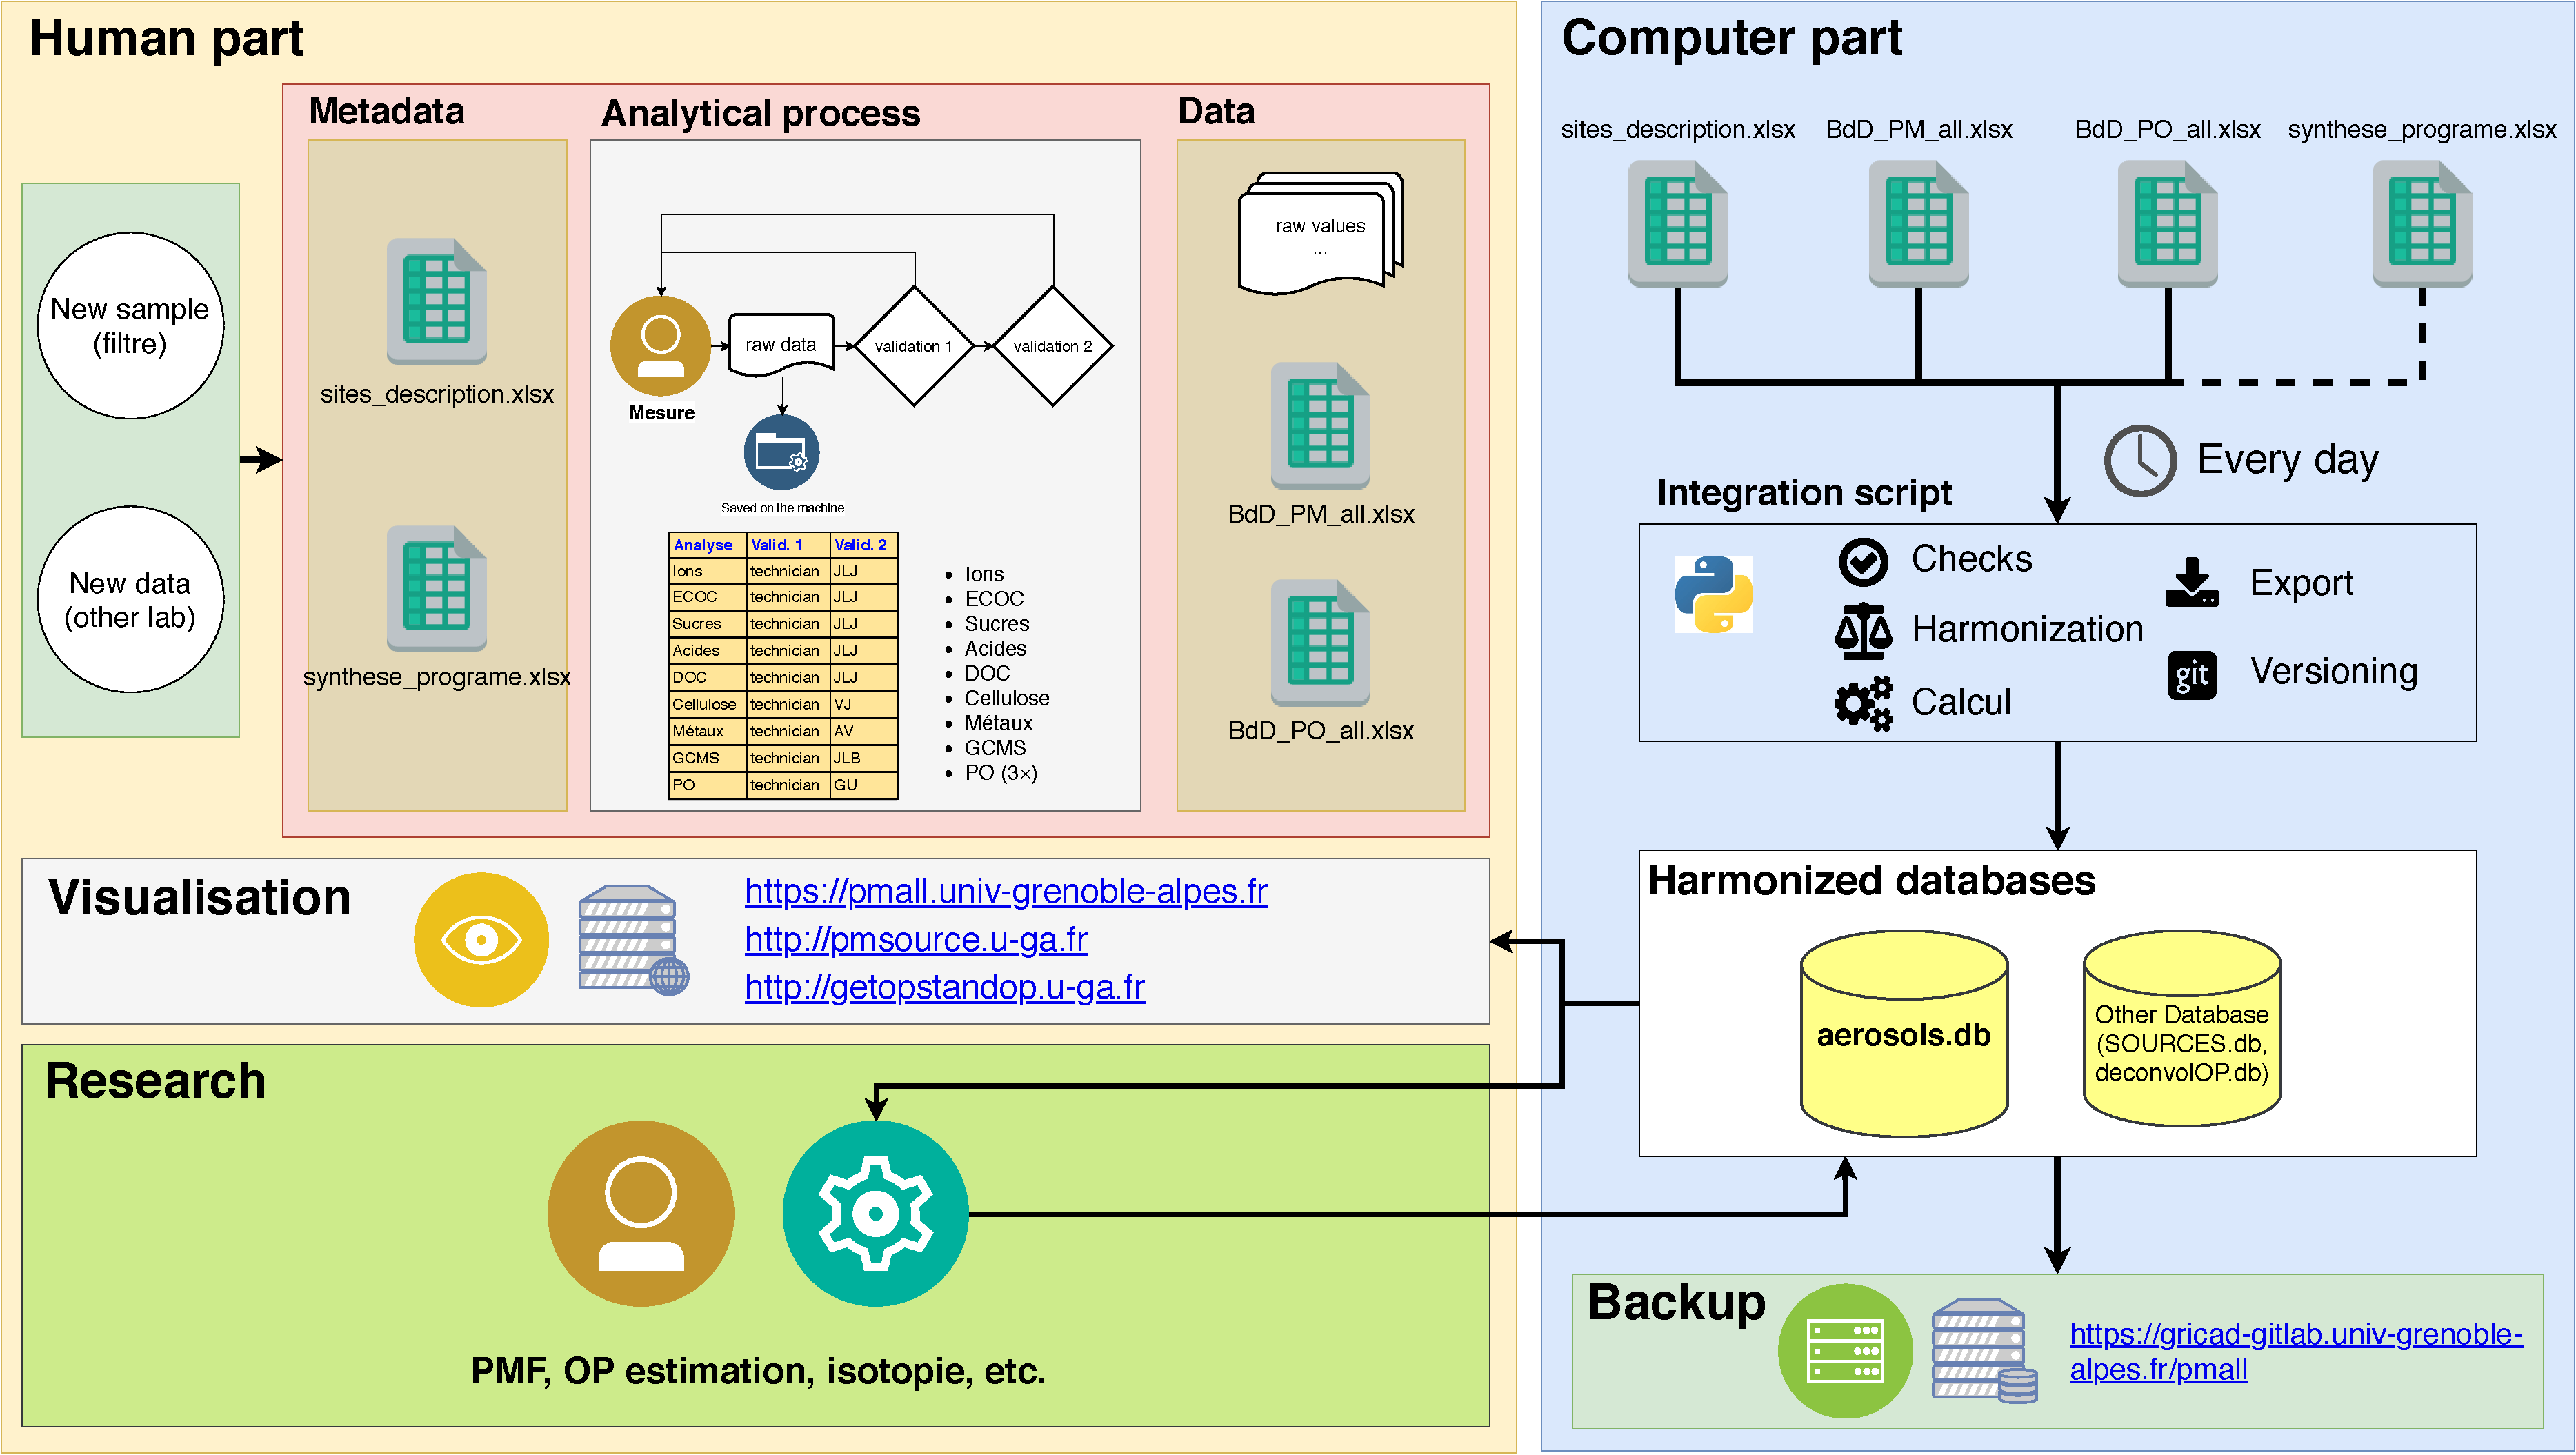
\includegraphics[width=\linewidth]{chapter02/workflow_simple.pdf}
    \caption{Vie d'un échantillon et des données : réception, analyse et enregistrement
        dans la filtrothèque et visualisation, puis utilisation dans les différents
        programmes de recherche.}%
    \label{fig:bdd}
\end{figure}
\end{landscape}

\subsection{Visualisation facilitée}%
\label{sub:visualisation_facilité}

La mise en place d'une interface de visualisation simple et rapide permet une première
exploration facilitée et centralisée en un même lieu
(voir~\ref{fig:figures/chapter02/pmall_example}). Aussi, le croissement de différentes
variables (lieu de prélèvement, espèces chimiques, sources issues des études PMF, mesure
du potentiel oxydant, variables météorologiques, etc.) est grandement simplifié.  De même,
cet outil est évolutif et des fonctionnalités peuvent être très facilement ajoutées. À la
simple évolution temporelle s'est ajoutée la dispersion et moyenne saisonière et mensuelle
ou encore la corrélation entre variable.

Ces différentes étapes de visualisation ne se substituent pas à un travail d'analyses
appronfondi, mais facilitent l'analyse exploratoire et la détection d'erreurs éventuelles.

\begin{figure}[ht]
    \centering
    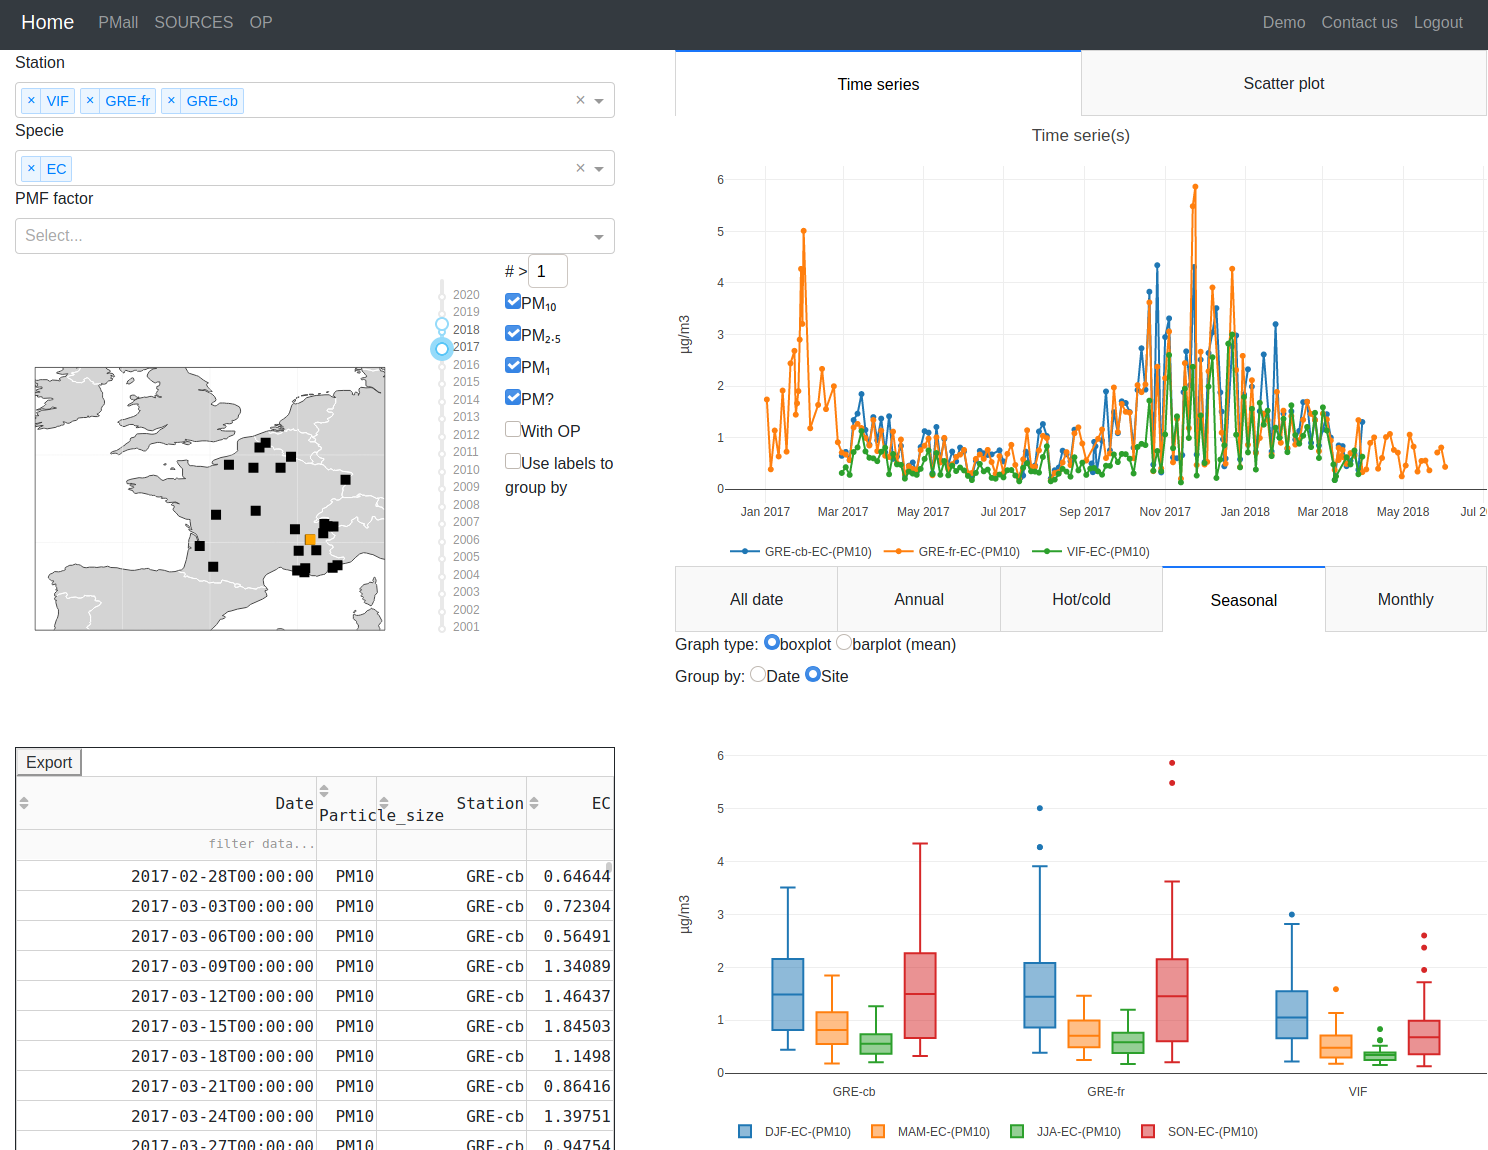
\includegraphics[width=1.0\linewidth]{figures/chapter02/pmall_example.png}
    \caption{Example d'utilisation de l'interface de visualisation de PMall.}%
    \label{fig:figures/chapter02/pmall_example}
\end{figure}


Après avoir présenté dans ce chapitre les différents outils et concepts utilisés ou
développés dans ce travail de thèse, les chapitres suivants vont s'attacher à présenter
les résultats sur les avancées de la déconvolution des sources de PM en ce qui concerne
les contributions massiques
(chapitre~\ref{cha:approfondissement_des_connaissances_des_sources_des_pm}) et les
contributions au potentiel oxydant (chapitre~\ref{cha:estimation_des_sources_de_PO}).




